\chapter{List coloring}

Firstly we can see a graph $G$ and its normal coloring which is depicted on a picture \ref{classic-coloring}. Whereas the list coloring shown on picture \ref{list-coloring} is that each vertex has a assigned list for which we can choose colors. Otherwise the coloring is the same.

\begin{figure}[!ht]
	\begin{subfigure}{0.45\textwidth}\centering
		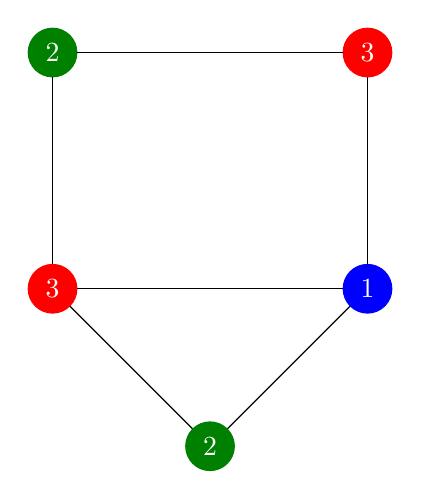
\begin{tikzpicture}[main/.style = {draw, circle, fill}]
			\node[main, color = Green] (1) at (0,0) {\textcolor{white}{2}};
			\node[main, color = Red] (2) at (-2,2) {\textcolor{white}{3}};
			\node[main, color = Blue] (3) at (2,2) {\textcolor{white}{1}};
			\node[main, color = Green] (4) at (-2,5) {\textcolor{white}{2}};
			\node[main, color = Red] (5) at (2,5) {\textcolor{white}{3}};
			\draw (1) -- (2);
			\draw (1) -- (3);
			\draw (2) -- (3);
			\draw (3) -- (5);
			\draw (2) -- (4);
			\draw (4) -- (5);
		\end{tikzpicture}
		\caption{Normal coloring of a graph $G$.}
		\label{classic-coloring}
	\end{subfigure}
	\begin{subfigure}{0.5\textwidth}\centering
		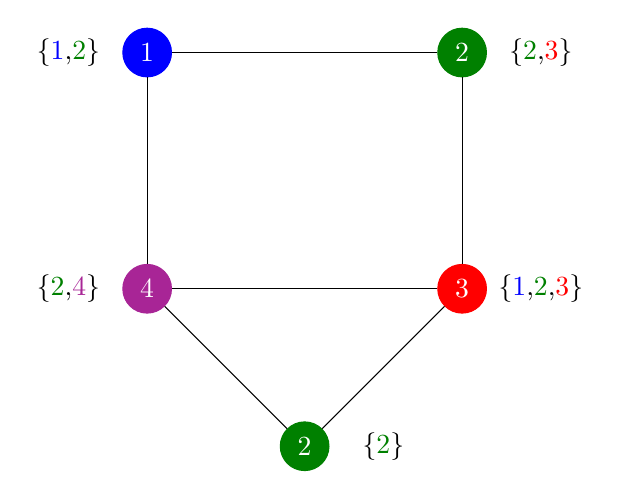
\begin{tikzpicture}[main/.style = {draw, circle, fill}]
			\node[main, color = Green] (1) at (0,0) {\textcolor{white}{2}};
			\node at (1,0) {\{\textcolor{Green}{2}\}};
			\node[main, color=Mulberry] (2) at (-2,2) {\textcolor{white}{4}};
			\node at (3,2) {\{\textcolor{Blue}{1},\textcolor{Green}{2},\textcolor{Red}{3}\}};
			\node[main, color = Red] (3) at (2,2) {\textcolor{white}{3}};
			\node at (-3,2) {\{\textcolor{Green}{2},\textcolor{Mulberry}{4}\}};
			\node[main, color = Blue] (4) at (-2,5) {\textcolor{white}{1}};
			\node at (3,5) {\{\textcolor{Green}{2},\textcolor{Red}{3}\}};
			\node[main, color = Green] (5) at (2,5) {\textcolor{white}{2}};
			\node at (-3,5) {\{\textcolor{Blue}{1},\textcolor{Green}{2}\}};
			\draw (1) -- (2);
			\draw (1) -- (3);
			\draw (2) -- (3);
			\draw (3) -- (5);
			\draw (2) -- (4);
			\draw (4) -- (5);
		\end{tikzpicture}
		\caption{List coloring of a graph $G$.}
		\label{list-coloring}
	\end{subfigure}
	\caption{Difference between basic and list coloring of a graph $G$.}
\end{figure}

\begin{defn}
	\textbf{$k$-list-assignment} is for an assignment for all vertices of size $k$.
\end{defn}

\begin{defn}
	The graph is \textbf{$k$-list-colorable} if $G$ can be colored by every $k$-list-assign-\\ment.
\end{defn}

\begin{defn}
	\textbf{List chromatic number} of a graph $G$ is denoted as $\chi_l(G)$. That is the min $k$ s.t. $G$ is $k$-list-colorable.
\end{defn}

\begin{observ}
	$\chi(G) \leq \chi_l(G)$
\end{observ}

Now one could prove that the Heawood's formula works pretty much the same, thus $\chi_l(G) \leq \left\lfloor \frac{7 + \sqrt{24 g + 1}}{2} \right\rfloor$, but only if $g > 0$. On the other hand one can find a planar graph which has $\chi_l(G) > 4$, but it can be shown that for every planar graph $G$ the $\chi_l(G) \leq 5$ which was proven by Thomassen. Vizing's theorem will be shown and the Brooks' theorem remains the same.

\begin{defn}
	$L$ is a \textbf{degree-list-assignment} for graph $G$ if $|L(v)| \geq \deg(v)$ $\forall v \in V$. And $G$ is a \textbf{degree-list-colorable} if $G$ is colorable from every degree-list-assignment.
\end{defn}

\begin{defn}[Gallai tree]
	\textbf{Gallai tree} is a graph where each 2-connected block is either a clique or an odd cycle.
\end{defn}

\begin{figure}[!ht]\centering
	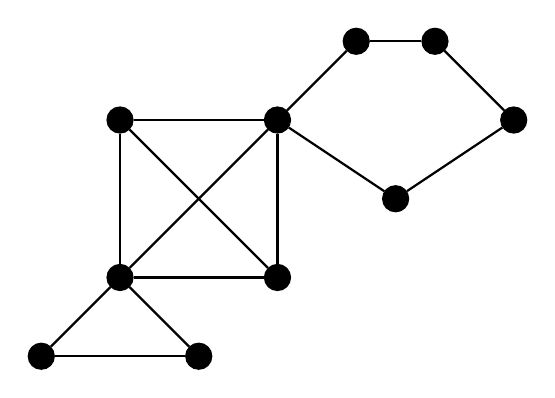
\begin{tikzpicture}[main/.style = {draw, circle, fill}, e/.style = {thick}]
		\node[main] (k4-1) at (0,0) {};
		\node[main] (k4-2) at (0,2) {};
		\node[main] (k4-3) at (2,0) {};
		\node[main] (k4-4) at (2,2) {};
		% K4-1 is C3-1
		\node[main] (c3-2) at (1,-1) {};
		\node[main] (c3-3) at (-1,-1) {};
		% K4-4 is C5-1
		\node[main] (c5-2) at (3,3) {};
		\node[main] (c5-3) at (4,3) {};
		\node[main] (c5-4) at (5,2) {};
		\node[main] (c5-5) at (3.5,1) {};
		\path[e] (k4-1) edge (k4-2) (k4-1) edge (k4-3) (k4-1) edge (k4-4)
			(k4-2) edge (k4-3) (k4-2) edge (k4-4) (k4-3) edge (k4-4);
		\path[e] (k4-1) edge (c3-2) (c3-2) edge (c3-3) (c3-3) edge (k4-1);
		\path[e] (k4-4) edge (c5-2) (c5-2) edge (c5-3) (c5-3) edge (c5-4) (c5-4) edge (c5-5) (c5-5) edge (k4-4);
	\end{tikzpicture}
	\caption{Example of a gallai tree.}
\end{figure}

\begin{observ}
	Gallai trees are not degree-list-colorable.
\end{observ}

\begin{thm}[Brooks]
	If $G$ is connected and $G$ is not a gallai tree then $G$ is degree-list-colorable.
\end{thm}

\begin{proof}
	\begin{lemma}
		$G$ is connected, $L$ is a degree-list-assignment $(\exists v \in V(G)) \ |L(v)| > \deg(v) \Rightarrow G$ is $L$-colorable.
	\end{lemma}
	
	\begin{lemma}
		$G$ is connected, $L$ is a degree-list-assignment, $uv \in E(G)$, $u$ is not a cut vertex, $G$ not $L$-colorable then $L(u) \subseteq L(v)$.
	\end{lemma}
	
	\begin{cor}
		$G$ connected, $L$ is a degree-list-assignment, $uv \in E(G)$, $u,v$ not cut vertices, $G$ not $L$-colorable then $L(u) = L(v)$.
	\end{cor}
	
	\begin{cor}
		$G$ is 2-connected, $L$ is degree-list-assignment, $G$ is not $L$-colorable then $\forall u,v \in V(G) : L(u) = L(v)$ and $G$ is a clique or an odd cycle.
	\end{cor}
\end{proof}

\TODO{From this part it is missing.}